\newpage
\section{Unsupervised keypoint learning}

In order to build a map it is useful to extract features, or keypoints, from images. Every keypoints should have a unique descriptor which can be used to identify it in the map which makes it possible to expand the map and also localize the camera. How to build a map and localize in it is out of scope for this thesis. This section will describe an unsupervised learning method to extract keypoints from images that would be usable in a full SFML pipeline.

The method evaluated in this thesis is based on the UnsuperPoint paper \cite{unsuperpoint} from 2019. The network architecture is illustrated in Figure \ref{fig:unsuperpoint}. The input image is fed into a shared backbone. The features from the backbone are then split into three different encoders that estimate the score, position and a descriptor for each keypoint. The network will estimate a keypoint in every $8\times 8$ patch of the image, but only the top $N$ keypoints sorted by score are used in the evaluation.

\begin{figure}[H]
	\centering
	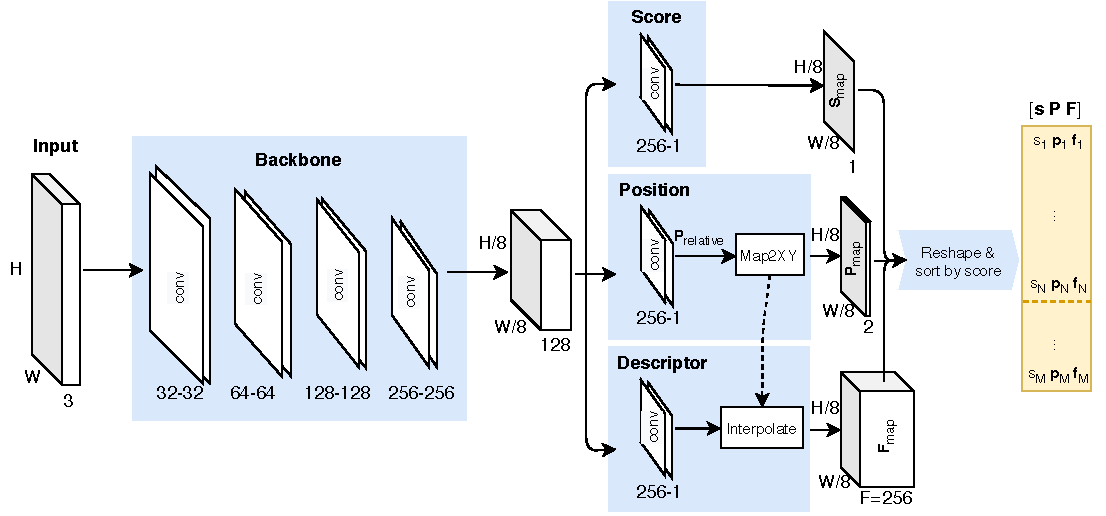
\includegraphics[width=1.0\textwidth]{unsuperpoint}
	\caption{The network has a common backbone and then splits into separate score, position and descriptor encoders. The output is reshaped and sorted by descending score.}
	\label{fig:unsuperpoint}
\end{figure}

The network is trained in a siamese twin setup, where two duplicate networks that share weights are fed different inputs and the loss is formulated by comparing the output scores, positions and descriptors.

\begin{figure}[H]
	\centering
	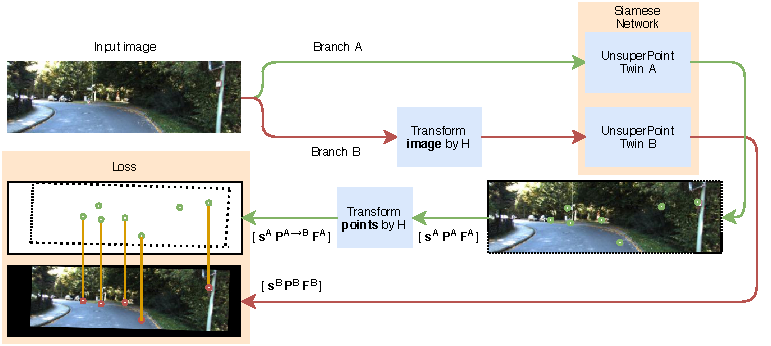
\includegraphics[width=1.0\textwidth]{unsuperpointloss}
	\caption{This figure illustrates the flow from input image to loss function. The image from branch A is fed directly into the UnsuperPoint network, while in branch B the image is first transformed by a random homography $H$. The keypoint positions from twin A are transformed by the same homography $H$ and the output from the two branches are compared in order to formulate the loss function.}
	\label{fig:unsuperpointloss}
\end{figure}

The score encoder is terminated by a sigmoid function and therefore predicts scores $s_n \in \mathbb{R} $ between 0 and 1 for each keypoint. The purpose of the scores are to rank the quality of the keypoints in all $8\times 8$px patches of the image and only pick the best ones. Typically patches in the sky and other non-textured areas will have keypoints with low scores.

The position encoder is also terminated by a sigmoid function and predicts the relative position of the keypoint in each patch. In the Map2XY block in Figure \ref{fig:unsuperpoint} the relative positions are converted to absolute pixel positions.

\[
P_{map,x}(r,c) = 8 * (c + P_{relative,x}(r,c))
\]
\[
P_{map,y}(r,c) = 8 * (r + P_{relative,y}(r,c))
\]

The descriptor encoder predicts a descriptor vector of length $F=256$ for each keypoint. The purpose of the descriptor is to find corresponding keypoints in different images. The constitutional layers produce 1 descriptor vector for each $8\times 8$ patch. This vector can be used directly as the keypoint descriptor and it works pretty well. Even better results can be achieved using the absolute keypoint positions to sample the values in the descriptor map with the same interpolation method used to do the warping in Figure \ref{fig:warp}.


\subsection{Loss function for keypoint learning}

Corresp G

pairs hat

dk

lposition

lsim

lscore

lunixy

ldesc

ldecorr



Brute force matching using PyTorch instead of OpenCV because we want to use the result as input to the next consensus step.